\chapter{ブレス攻撃時の表示方法}
\label{sec:display}

\section{表示方法の概要}

本研究では，VRゲームにおけるブレス攻撃時の視認性とゲーム体験に及ぼす影響を調査するため，4種類の表示条件を設定した．3種類はブレス攻撃エフェクトの表示方法を変更する条件であり，残りの1種類は攻撃対象となるオブジェクトの表示方法を変更する条件である．これらを比較することで，表示方法の違いが視認性とゲーム体験に及ぼす影響を調査する．

\section{各表示方法}

以下に各表示方法の概要を\figref{fig:3}と共に示す．

\begin{figure}[htbp]
  \centering
  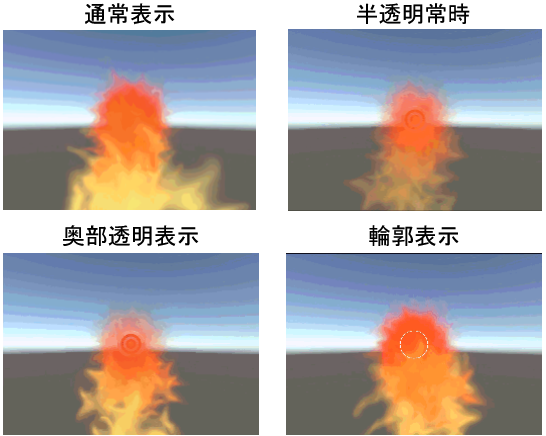
\includegraphics[width=0.8\linewidth]{fig/fire.png}
  \caption{各表示条件の比較}
  \label{fig:3}
\end{figure}

\begin{itemize}
    \item 通常表示：
    エフェクトを通常どおり表示する．ほかの表示方法と比較するための基準とする．

    \item 半透明表示：
    エフェクト全体を半透明にして表示する．エフェクト越しに攻撃対象を確認しやすくする．

    \item 奥部透明表示：
    エフェクトの奥側を透明にし，手前側は通常どおり表示する．エフェクトの一部のみ表示を変更することで，視認性とエフェクトの見た目の両立を図る．

    \item 輪郭表示：
    対象物の輪郭を表示し，エフェクトと重なった場合でも対象物の位置や形状を把握しやすくする．
\end{itemize}

これらの表示方法を比較することで，エフェクトによる遮蔽の軽減が視認性に及ぼす影響と，表示の変化がゲーム体験に及ぼす影響を調査する．